%%%%%%%%%%%%%%%%%%%%%%%%%%%%%%%%%%%%%%%%%%%%%%%%%%%%%%%%%%%%%%%%%%%%%%
% How to use writeLaTeX:
%
% You edit the source code here on the left, and the preview on the
% right shows you the result within a few seconds.
%
% Bookmark this page and share the URL with your co-authors. They can
% edit at the same time!
%
% You can upload figures, bibliographies, custom classes and
% styles using the files menu.
%
% If you're new to LaTeX, the wikibook is a great place to start:
% http://en.wikibooks.org/wiki/LaTeX
%
%%%%%%%%%%%%%%%%%%%%%%%%%%%%%%%%%%%%%%%%%%%%%%%%%%%%%%%%%%%%%%%%%%%%%%
\documentclass{tufte-handout}

%\geometry{showframe}% for debugging purposes -- displays the margins

\usepackage{amsmath}

% Set up the images/graphics package
\usepackage{graphicx}
\setkeys{Gin}{width=\linewidth,totalheight=\textheight,keepaspectratio}
\graphicspath{{graphics/}}

\title{Title}
\author{DIME staff \\ Development Impact Evaluation}
\date{11 June 2019}  % if the \date{} command is left out, the current date will be used

% The following package makes prettier tables.  We're all about the bling!
\usepackage{booktabs}

% The units package provides nice, non-stacked fractions and better spacing
% for units.
\usepackage{units}

% The fancyvrb package lets us customize the formatting of verbatim
% environments.  We use a slightly smaller font.
\usepackage{upquote}
\usepackage{fancyvrb}
\fvset{fontsize=\normalsize}
\renewcommand{\FancyVerbFormatLine}{\color{violet}}
\DefineShortVerb{\|}

% Small sections of multiple columns
\usepackage{multicol}

% Provides paragraphs of dummy text
\usepackage{lipsum}

% These commands are used to pretty-print LaTeX commands
\newcommand{\doccmd}[1]{\texttt{\textbackslash#1}}% command name -- adds backslash automatically
\newcommand{\docopt}[1]{\ensuremath{\langle}\textrm{\textit{#1}}\ensuremath{\rangle}}% optional command argument
\newcommand{\docarg}[1]{\textrm{\textit{#1}}}% (required) command argument
\newenvironment{docspec}{\begin{quote}\noindent}{\end{quote}}% command specification environment
\newcommand{\docenv}[1]{\textsf{#1}}% environment name
\newcommand{\docpkg}[1]{\texttt{#1}}% package name
\newcommand{\doccls}[1]{\texttt{#1}}% document class name
\newcommand{\docclsopt}[1]{\texttt{#1}}% document class option name

\begin{document}
	
	\maketitle% this prints the handout title, author, and date
	
	\begin{marginfigure}%
		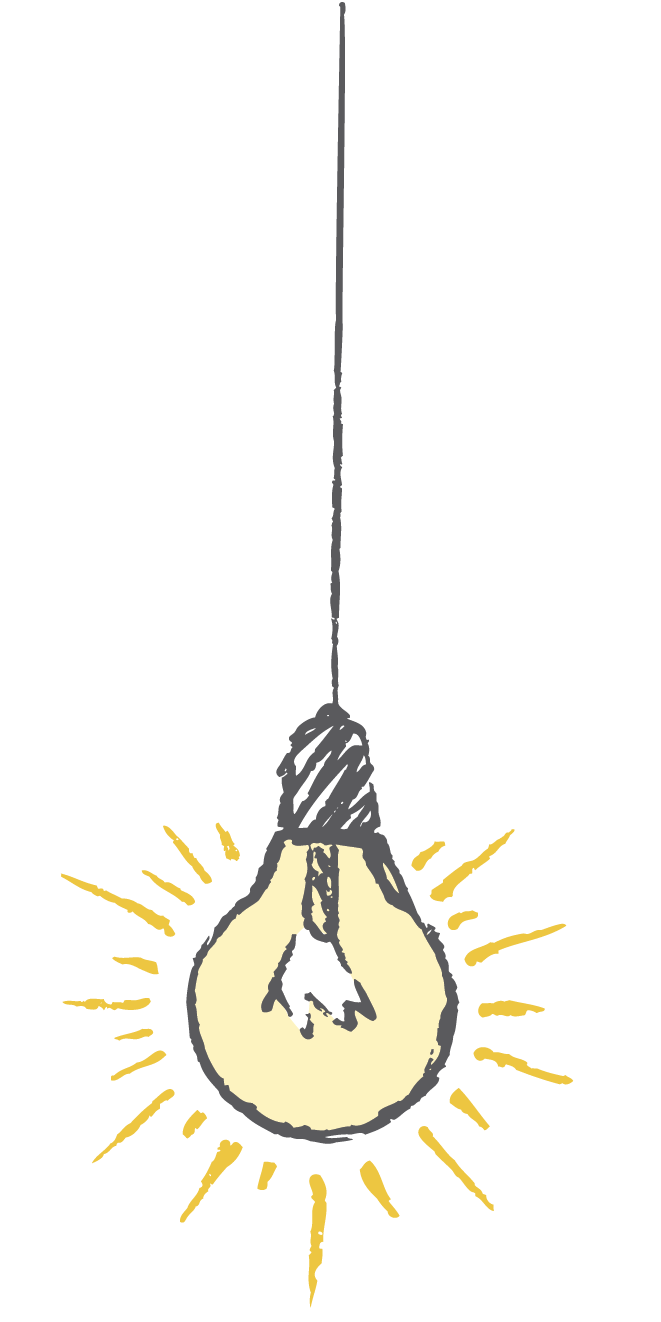
\includegraphics[width=\linewidth]{img/light.png}
	\end{marginfigure}
	
	\begin{abstract}
		Lorem ipsum dolor sit amet, consectetur adipiscing elit. Sed suscipit tortor quis dapibus cursus. Fusce et tempus dolor. Nunc sed libero in purus imperdiet sollicitudin non et libero. Nam sit amet sollicitudin dui. Ut semper auctor condimentum. Proin ut dignissim lectus. Vestibulum ante ipsum primis in faucibus orci luctus et ultrices posuere cubilia curae; Curabitur nec nisl eget nibh tincidunt mollis. Aenean facilisis ante quis purus condimentum, vel ullamcorper urna venenatis. Integer ut aliquam elit, ac dapibus lorem. Maecenas eu volutpat metus, et suscipit neque. Morbi rhoncus est ac fermentum consectetur. Nullam auctor interdum ex, vitae porta nulla porta sed. Phasellus quis magna in ligula molestie scelerisque vel id elit.
	\end{abstract}
	
	%\printclassoptions
	\section{Section title}
		
	Duis non elementum risus. Orci varius natoque penatibus et magnis dis parturient montes, nascetur ridiculus mus. Integer quis rhoncus lorem. Mauris a vulputate leo. Cras vel lectus quis arcu blandit pretium sit amet ac felis. Praesent ullamcorper scelerisque risus, id suscipit orci ultricies ut. Etiam enim enim, hendrerit nec purus id, euismod vehicula velit. Morbi blandit felis ut ex pretium, gravida tincidunt justo tristique. Sed feugiat ipsum nec tempus vehicula. Cras sit amet metus tellus. Morbi at dui risus. Ut auctor quis justo nec ultrices. Maecenas vestibulum nisi vitae tellus consectetur, at commodo tellus feugiat.
	
	Sed accumsan nisi lorem, a placerat nulla malesuada eu. Nam in sem ex. Curabitur auctor pulvinar massa nec convallis. Nullam sed lectus sit amet mauris vulputate lacinia. Ut gravida tortor nunc, ut ullamcorper leo placerat nec. Cras ullamcorper mollis feugiat. Proin facilisis tempus dolor, ut mattis dolor imperdiet ut. Curabitur et nibh nec enim suscipit sodales. Phasellus sagittis, dolor a viverra elementum, ligula augue pretium magna, eget porttitor mi arcu quis nunc. Vivamus gravida et neque eu mattis. Cras sollicitudin feugiat tortor vitae gravida. Aliquam erat volutpat.
		
	\begin{fullwidth}
		
		\section{Full width}
		
		Aenean consectetur leo eu malesuada mattis. Vivamus sit amet congue tortor. Etiam dapibus diam nec purus faucibus ultricies. Morbi eget volutpat diam. Suspendisse sed urna eu ante dictum molestie varius eget diam. Sed eleifend, nisl quis dapibus molestie, arcu mi elementum metus, et ullamcorper lacus quam vitae mauris. Curabitur non fringilla sapien. Sed mollis, lorem ac lacinia tempor, ligula lorem dignissim nibh, vitae tempus dolor tellus sed neque. Sed ut iaculis ex. Pellentesque vitae porttitor elit. Nullam interdum lorem erat, posuere viverra tortor sodales a. Proin luctus sapien a libero imperdiet, a molestie leo dictum. Maecenas sollicitudin velit semper leo ultrices, eget vehicula velit consequat. Praesent ut sodales nisl.
	
	\end{fullwidth}
	
	\section{Section title}
	
	Aenean consectetur leo eu malesuada mattis. Vivamus sit amet congue tortor. Etiam dapibus diam nec purus faucibus ultricies. Morbi eget volutpat diam. Suspendisse sed urna eu ante dictum molestie varius eget diam. Sed eleifend, nisl quis dapibus molestie, arcu mi elementum metus, et ullamcorper lacus quam vitae mauris. Curabitur non fringilla sapien. Sed mollis, lorem ac lacinia tempor, ligula lorem dignissim nibh, vitae tempus dolor tellus sed neque. Sed ut iaculis ex. Pellentesque vitae porttitor elit. Nullam interdum lorem erat, posuere viverra tortor sodales a. Proin luctus sapien a libero imperdiet, a molestie leo dictum. Maecenas sollicitudin velit semper leo ultrices, eget vehicula velit consequat. Praesent ut sodales nisl.
		
	
	
\end{document}